\section{Nonlinearity Index Scaling}

Figure \ref{fig:p-sweep} illustrates the computational cost across distinct physical regimes by sweeping the power index \(p\) from 1.5 to 4.0. The grid resolution is fixed at \(N_x = 1000\) with a solver tolerance of \(10^{-6}\) and a regularization parameter of \(\varepsilon = 10^{-6}\). The remaining parameter is fixed at \(T = 0.05\).

All three solvers hit their absolute performance floor at the \(p=2.0\) mark. This behavior is mathematically expected: at \(p=2\), the nonlinearity vanishes entirely, reducing the system to the standard, linear heat equation. The system Jacobian becomes constant, requiring minimal updates. For instance, the BDF solver solves the \(p=2.0\) case in a mere 0.04 seconds, needing only a single Jacobian evaluation across the entire simulation time.

Moving away from the linear baseline exposes severe differences in solver efficiency. In the singular regime (\(p < 2\)), execution times rise moderately as the diffusion coefficient attempts to diverge in regions with flat gradients. However, the true stress test occurs in the degenerate regime (\(p > 2\)). Here, the diffusion term approaches zero where the gradient is small, generating sharp, slow-moving spatial fronts that force solvers to take microscopic time steps. 

BDF and Radau degrade severely as \(p\) scales up. At \(p=4.0\), BDF requires 11.2 seconds to resolve the physics, while Radau struggles for 14.2 seconds, forcing an immense 38,201 function evaluations and 2,122 Jacobian updates to push through the stiffness. In stark contrast, LSODA navigates the degenerate regime with remarkable efficiency. Even at the highly nonlinear \(p=4.0\) limit, LSODA completes the integration in just 0.54 seconds. Its internal heuristics clearly manage the sharp shifting gradients better than the pure implicit methods. This widens the performance gap by over an order of magnitude at the extremes of the parameter space.

\begin{figure}[H]
  \centering
  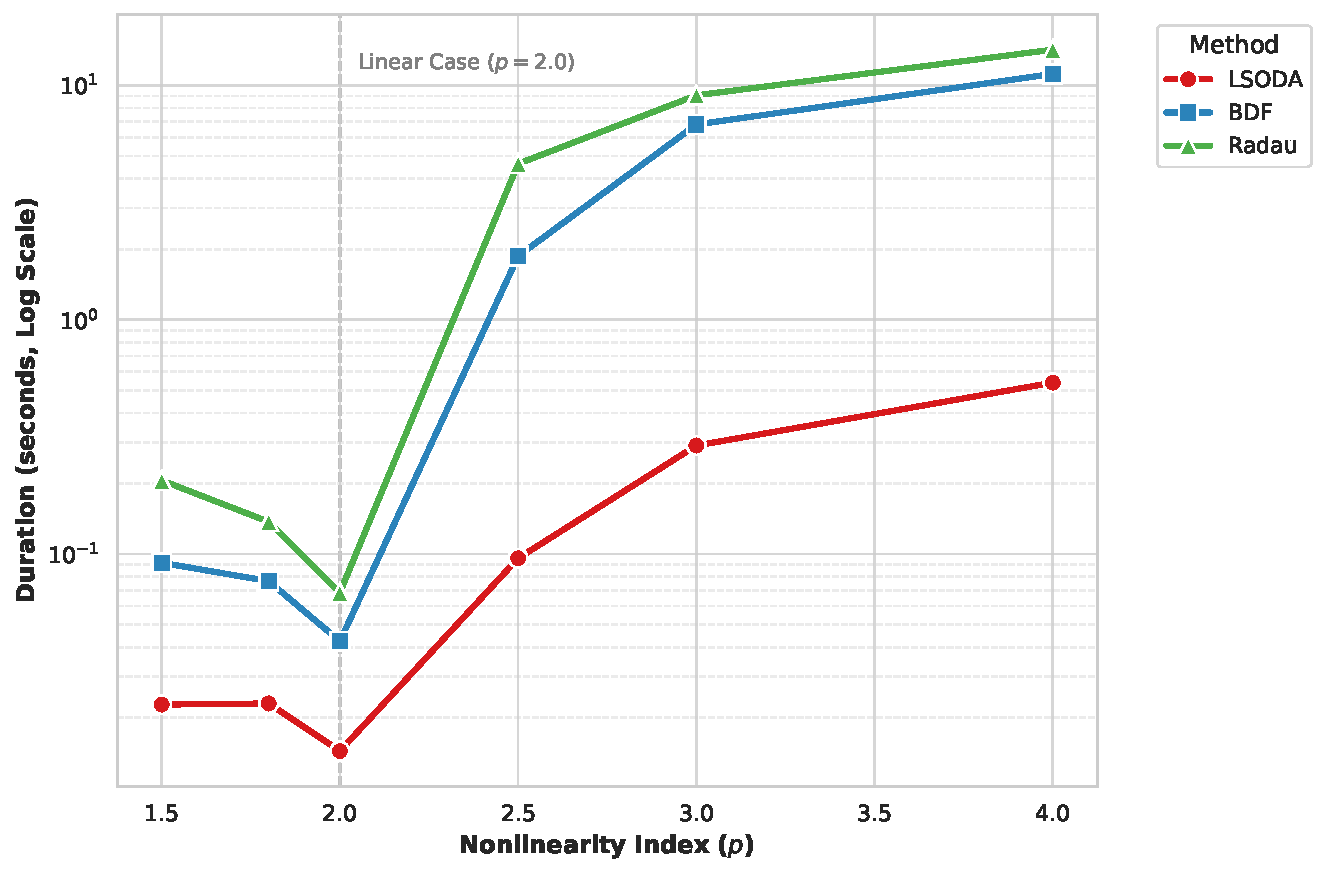
\includegraphics[width=\textwidth]{images/p_sweep.pdf}
  \caption{Execution time scaling of LSODA, BDF, and Radau solvers against the nonlinearity index \(p\).}
  \label{fig:p-sweep}
\end{figure}
